\chapter{Specifikt för Kårspexet 25/26}
\section{Gitarr \& Bas}
Gitarr kan noteras med TAB, med noter, eller komp-notation (ackord och eventuell rytm). Valet ligger hos arrangören och beror på detaljnivån med vilken man vill beskriva gitarrstämman. 

Bas kan noteras med noter eller komp-notation.


\section{Keyboard}
Keyboardstämmor kan noteras med noter, komp-notation, eller komp-notation med en utskriven melodilinje. För stämmor med ett ljud med ett tydligt anslag (exempelvis piano) rekommenderas helt utskrivna noter, medan komp-notation kan passa bättre för orgel- och syntstämmor där inte stämmans exakta utförande är lika viktigt.


I keyboardstämmor finns det möjlighet att anpassa instrumentljudet. Ljudändringar markeras med understruken text ovanför stämman. Texten ska vara kort och beskrivande (ex. ``\underline{Såg-synt}", ``\underline{80s brass}", ``\underline{Marimba}"). Vissa keyboards har möjlighet att dela upp tangentbordet och spela olika ljud i höger och vänster hand. Denna funktionalitet bör inte antagas finnas, men om den bekräftats och ska notsättas markeras detta med ``\underline{RH: \textit{höger hands ljud}, LH: \textit{vänster hands ljud}}", t.ex. ``\underline{RH: Piano, LH: Square bass}".

\vspace{1em}
I orkestern för Kårspexet 25/26 finns en elorgel. Denna noteras på tre rader, där de två övre (höger och vänster hand) är sammanbunda och den nedersta (fötter) är frikopplad. Raderna har klaverna G-klav, F-klav, F-klav. Ljudinställningar och manualfördelningar rekommenderas att lämnas till instrumentalist och kapellmästare såvida arrangören inte har egen orgelexpertis eller mycket starka åsikter om den exakta ljudbilden. 

Då orgelinställningar ska noteras används \verb|I.| och \verb|II.| för manualer, och \verb|Pd.| för pedaler. Drawbar-inställningar noteras ``\underline{XXXXXXXX}'' där X är siffror 0 till 8, ex. ``\underline{88405062}"

\begin{center}
    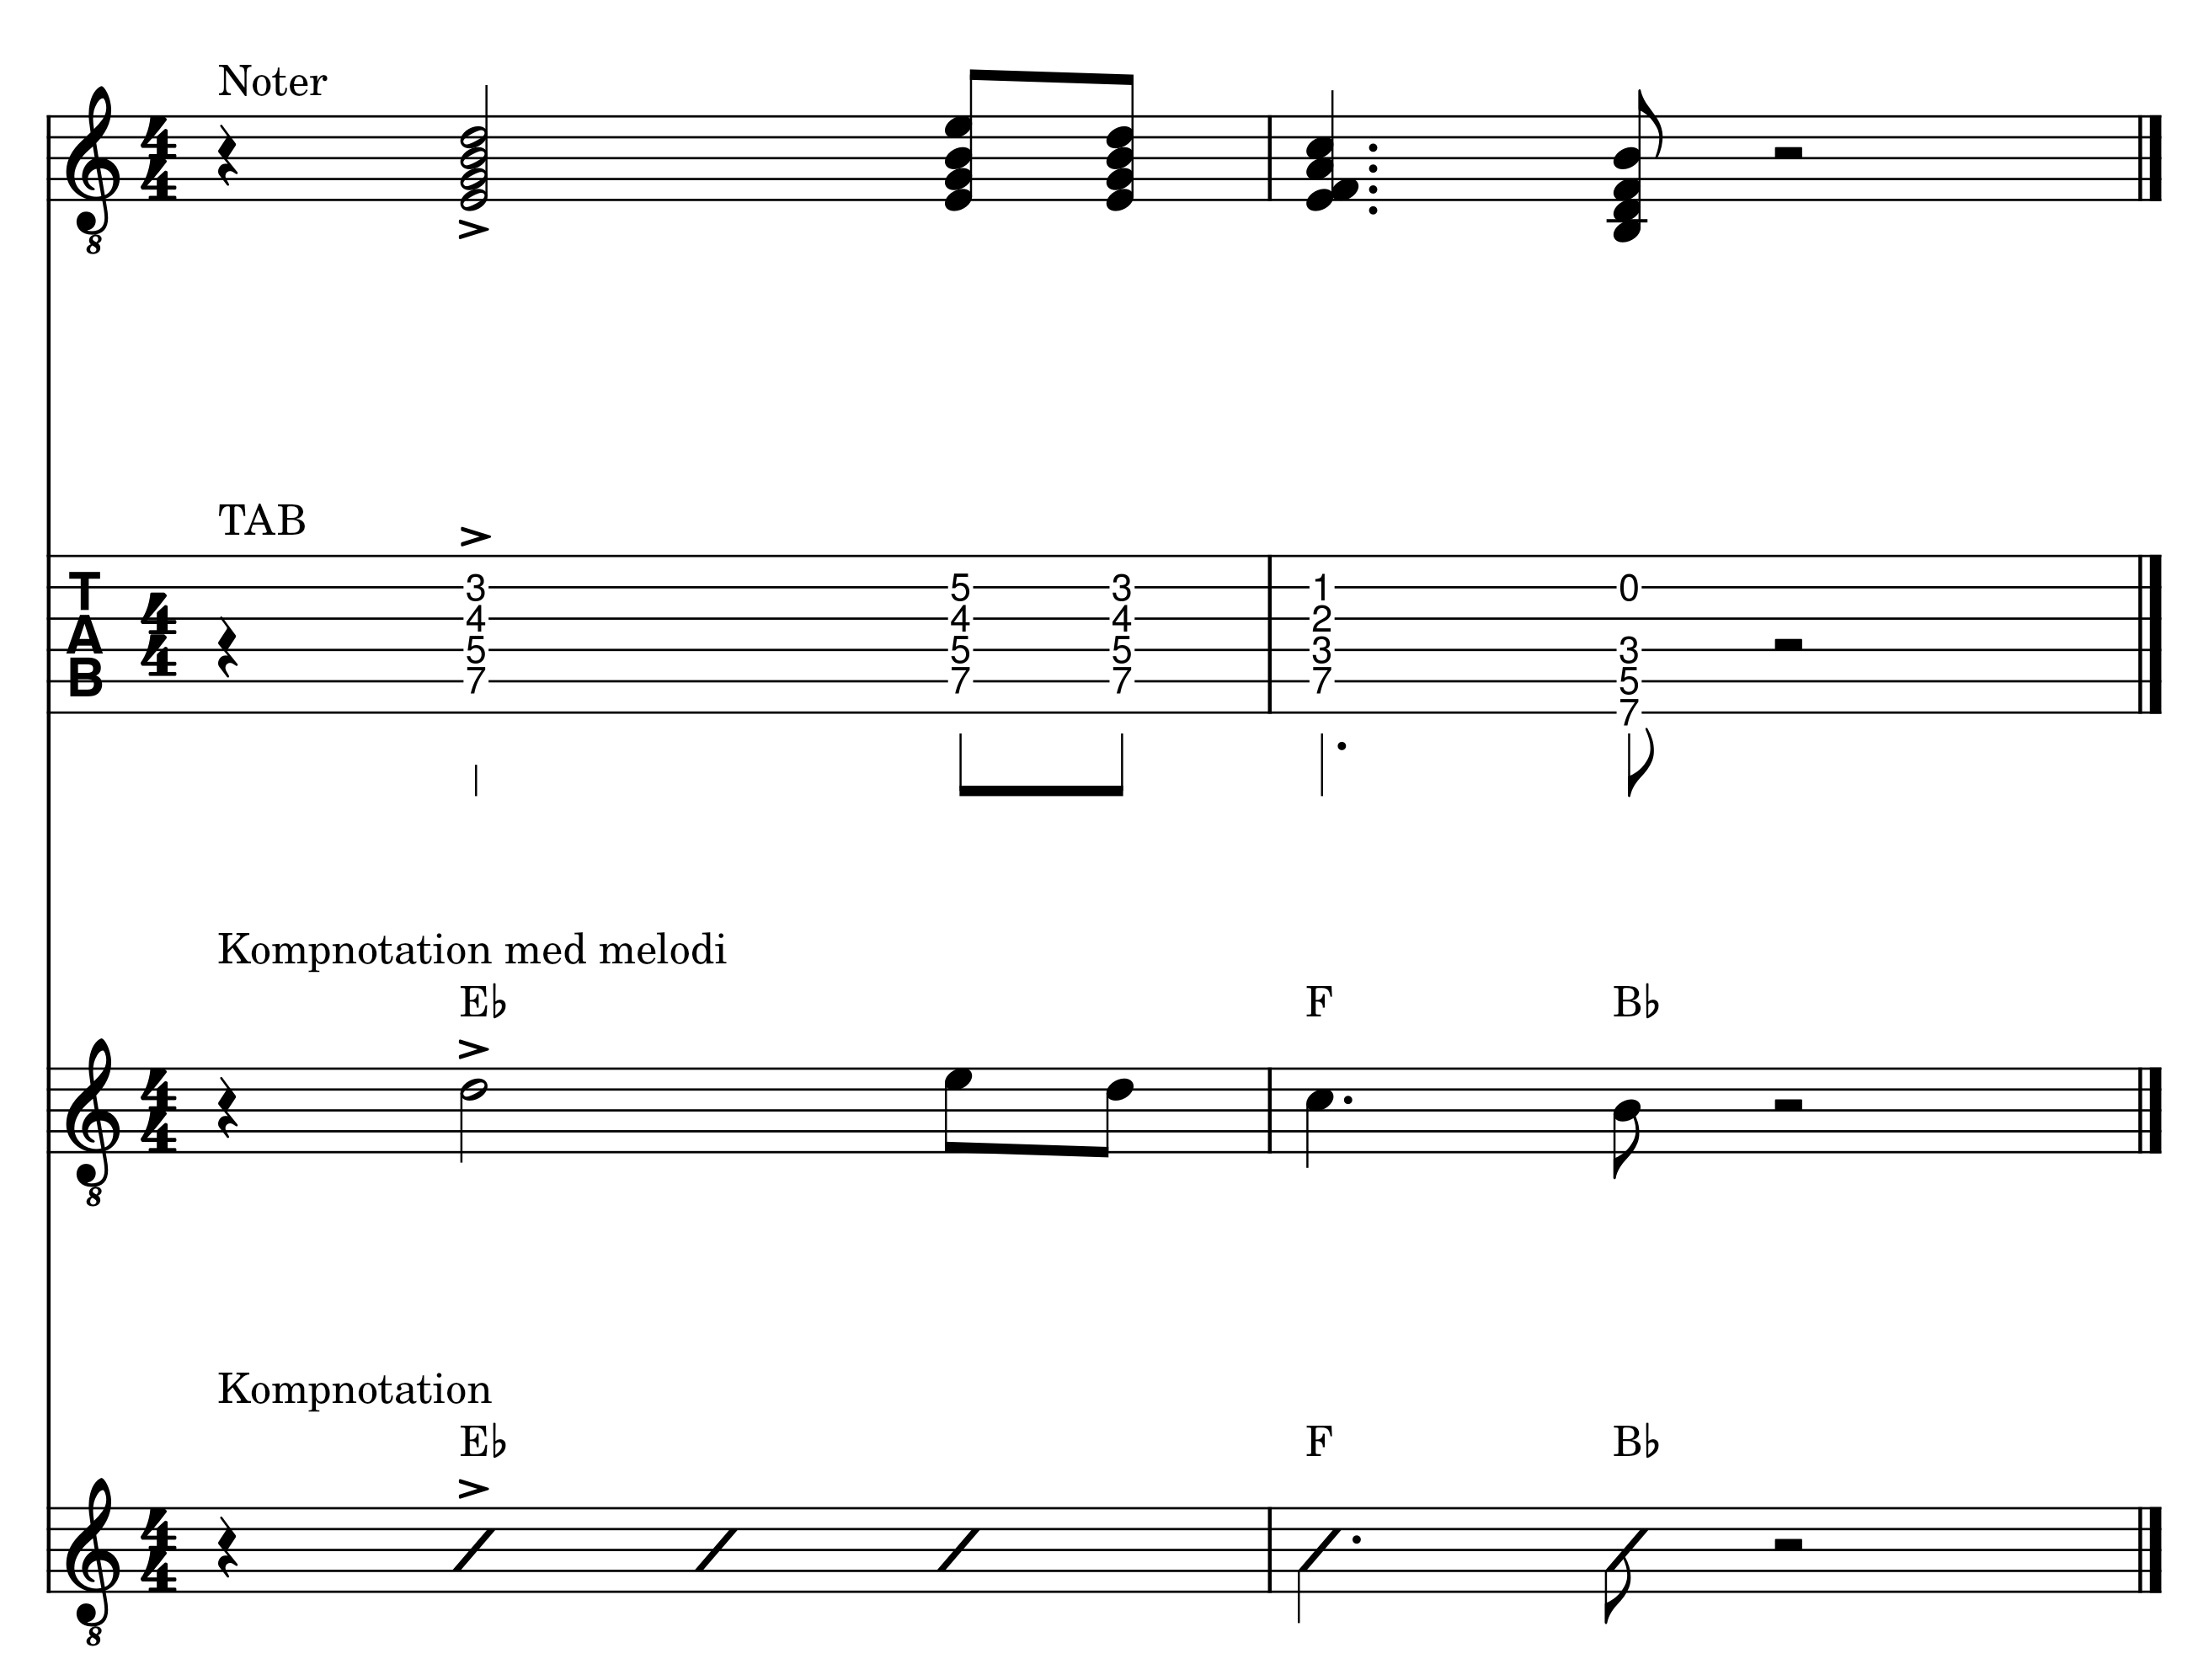
\includegraphics[width=\textwidth]{lilypond/kompnotation.cropped.png}
\end{center}

\section{Kapellmästare}
Kapellmästaren läser omväxlande från sin egen stämnot och från partituret. Kapellmästarens exemplar av partituret är generellt utskrivet i A4-storlek, direkt nedskalad från A3. Det lättaste sättet att lämna anteckningar och kommentarer är att sätta text i stämmorna för de instrument som kommentaren rör. Om kommentaren gäller hela orkestern ska den sättas som system-text, så att alla stämmor ser den. Om kommentaren enbart rör kapellmästaren och inte resten av orkestern ska den sättas i kapellmästarens egen stämma. 

I Kårspexet 25/26 spelar kapellmästaren keyboard, i partituret benämnt Keyboard 0. Keyboard 0 behöver inte alltid spela; om någon keyboard-stämma saknar en stämma i ett arr ska det vara Keyboard 0. Om musiken är rytmiskt krånglig och/eller fluktuerande, eller kräver direktreaktion till skådis kan Keyboard 0 utelämnas eller ges en relativt enkel (enhändig) stämma för att lämna plats för ledandet av orkestern. Keyboard 0 bör dock också användas då en (solo) pianostämma kräver timing och kontakt med skådis (ex. Colla Voce eller små Vamps), för att minska mellanhänderna i tempoändringar. Keyboard 0 passar också bra för små korta insatser då och då, t.ex. slagverk eller ljudeffekter.
